\documentclass[../../main]{subfiles}
\begin{document}

\subsection{Friends}
\label{ss:final-friends}
As said earlier this app implement also a social context by allowing the users to send/deny/confirm friend request from other users. Thanks to this
a user is not only limited on his poi but he can see, add or be notified on the public poi of his friends.
There are many action that a user can perform on this context starting from his friends list and send a friend request as shown in the next picture.
\begin{figure}[H]
    \centering
    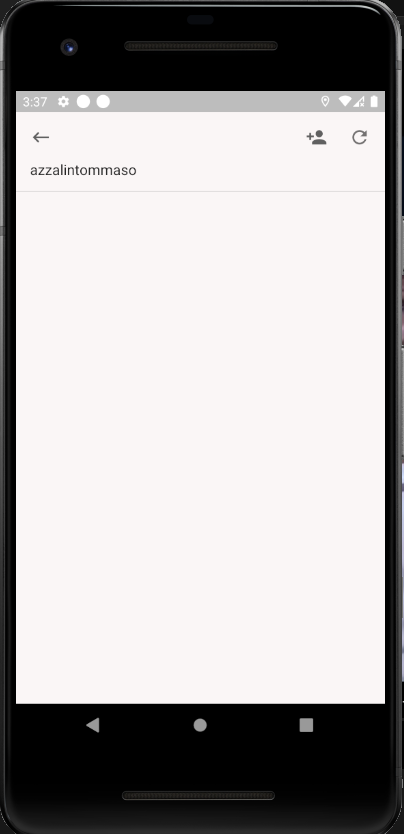
\includegraphics[width=70mm,height=150mm]{images/app/friend/friend_overwiew.png}
    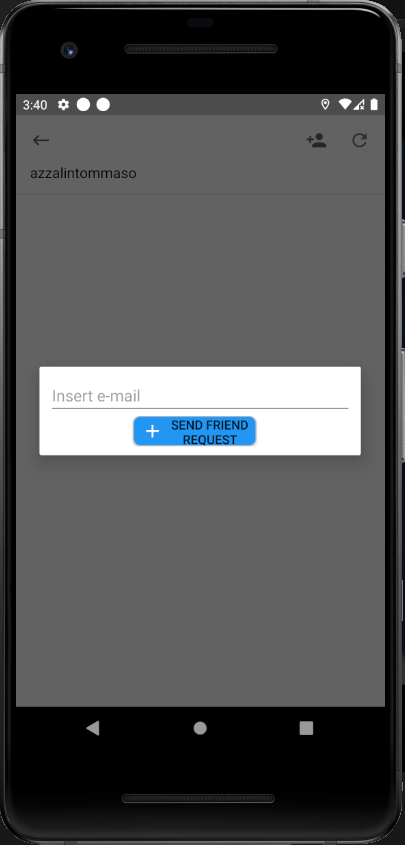
\includegraphics[width=70mm,height=150mm]{images/app/friend/send_request.png}
    \caption{On the left the overview of friends list and on the right the dialog to send a frienship request.}
\end{figure}

To accept or deny a friendship request a dialog pop up after clicking the apposite notification, and when a user confirm it the sender receive the notification.
An example is the one listed here.

\begin{figure}[H]
    \centering
    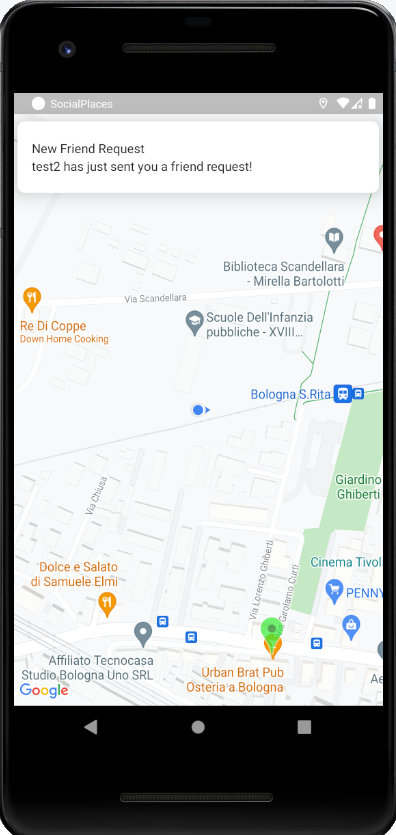
\includegraphics[width=50mm,height=120mm]{images/app/notification/friend/friend_request_notification.png}
    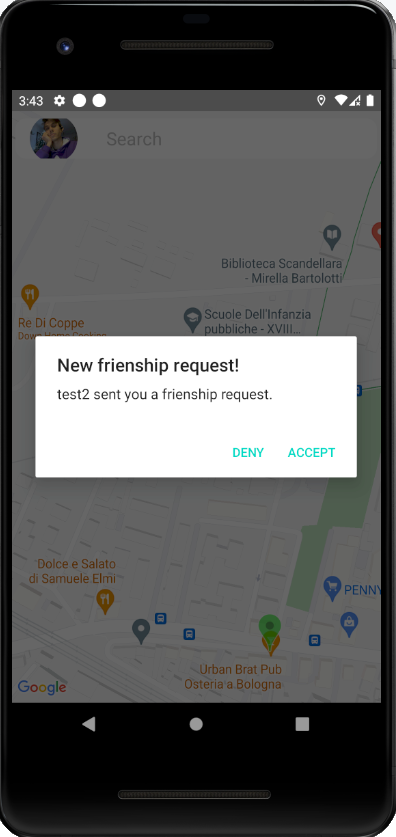
\includegraphics[width=50mm,height=120mm]{images/app/notification/friend/dialog_friend_request.png}
    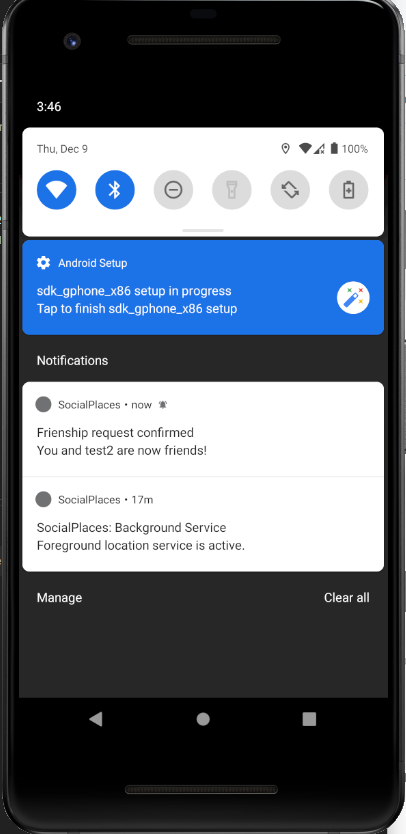
\includegraphics[width=50mm,height=120mm]{images/app/notification/friend/confirmed_request.png}
    \caption{On the left the notification of a friend request, center the dialog to accepty/deny it and on the right the notification of a confirmed friendship request.}
\end{figure}
\newpage
Naturally a user can see the public poi of his friend and add it to his personal poi as shown in this figure:
\begin{figure}[H]
    \centering
    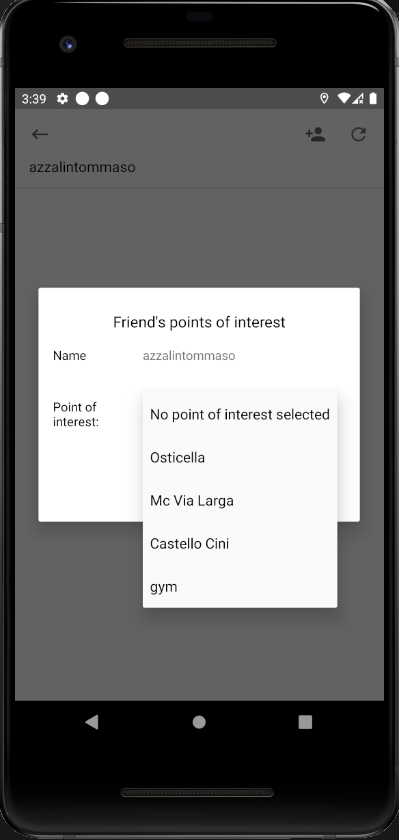
\includegraphics[width=70mm,height=150mm]{images/app/friend/friend_poi.png}
    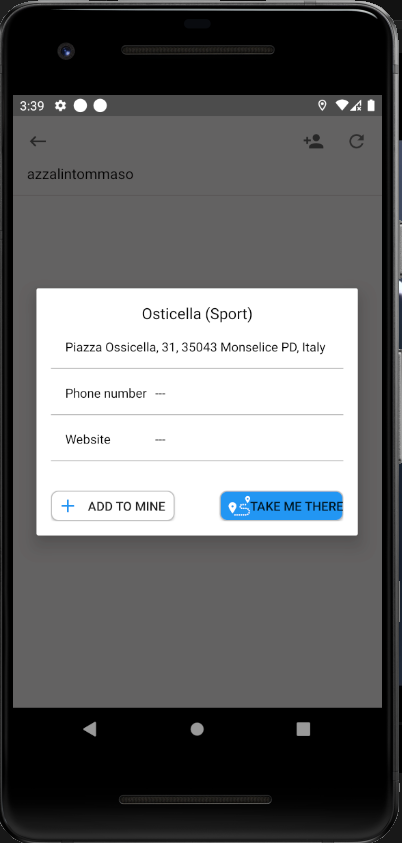
\includegraphics[width=70mm,height=150mm]{images/app/friend/add_friend_poi.png}
    \caption{On the left the list of the public poi of user's friend and on the right the dialog to add a poi to user's personal list.}
\end{figure}

\end{document}